\documentclass[11pt]{article}


\usepackage[margin=1in,a4paper]{geometry}
\usepackage[utf8]{inputenc}
\usepackage[T1]{fontenc}
\usepackage{lmodern}
\usepackage{tabularx}
\usepackage{quoting}
\usepackage{fancyhdr}
\usepackage{graphicx}
\usepackage{nicefrac}
\usepackage{sectsty}
\usepackage{graphicx}
\usepackage[T1]{fontenc}
\usepackage{epigraph} %quotes
\usepackage{amssymb} %math symbols
\usepackage{mathtools} %more math stuff
\usepackage{amsthm} %theorems, proofs and lemmas
\usepackage{optidef} %fast optimization problem notation
\usepackage{changepage}
\usepackage{gensymb}
\usepackage[ruled,vlined,noend,linesnumbered]{algorithm2e} %algoritms/pseudocode


\usepackage{biblatex}

%% asmthm notation
\newtheorem{theorem}{Theorem}[section]
\newtheorem{corollary}{Corollary}[theorem]
\newtheorem{lemma}[theorem]{Lemma}
\newtheorem{problem}{Problem}
\newtheorem{definition}{Definition}
\newtheorem{claim}{Claim}[section]


%% declaring abs so that it works nicely
\DeclarePairedDelimiter\abs{\lvert}{\rvert}%
\DeclarePairedDelimiter\norm{\lVert}{\rVert}%

\let\oldnl\nl% Store \nl in \oldnl
\newcommand{\nonl}{\renewcommand{\nl}{\let\nl\oldnl}}% Remove line number for one specific line in algorithm

\title{BIOENG-404 - Homework 4: SCONE}
\author{
    Titouan Renard
    - MT : Robotics 
}
\date{\today}



\begin{document}


\maketitle

\section{Healthy Gait}

The solution provided by the optimization process (which converges relatively fast) is quite good. The gait appears natural when played as a video but a close examination of the gait parameters (pelvic tilt, hip, knee and ankle flexion as well as ground reaction forces, displayed in figure \ref{healthy_gait}) show that the model gives results slightly off compared to measured data in humans. The curves have the approximate shape of the real-life data but their amplitude and timing is slightly off. Furthermore one observes that the ankle flexion displays a dip in angle at $\sim 25\%$ of the gait cycle that simply doesn't exist in humans. This model seems more useful as a toy-model, to rapidly test out hypotheses rather than as an accurate prediction tool (as is often the case when modeling complex dynamical systems).

\begin{figure}[h!]
    \centering
    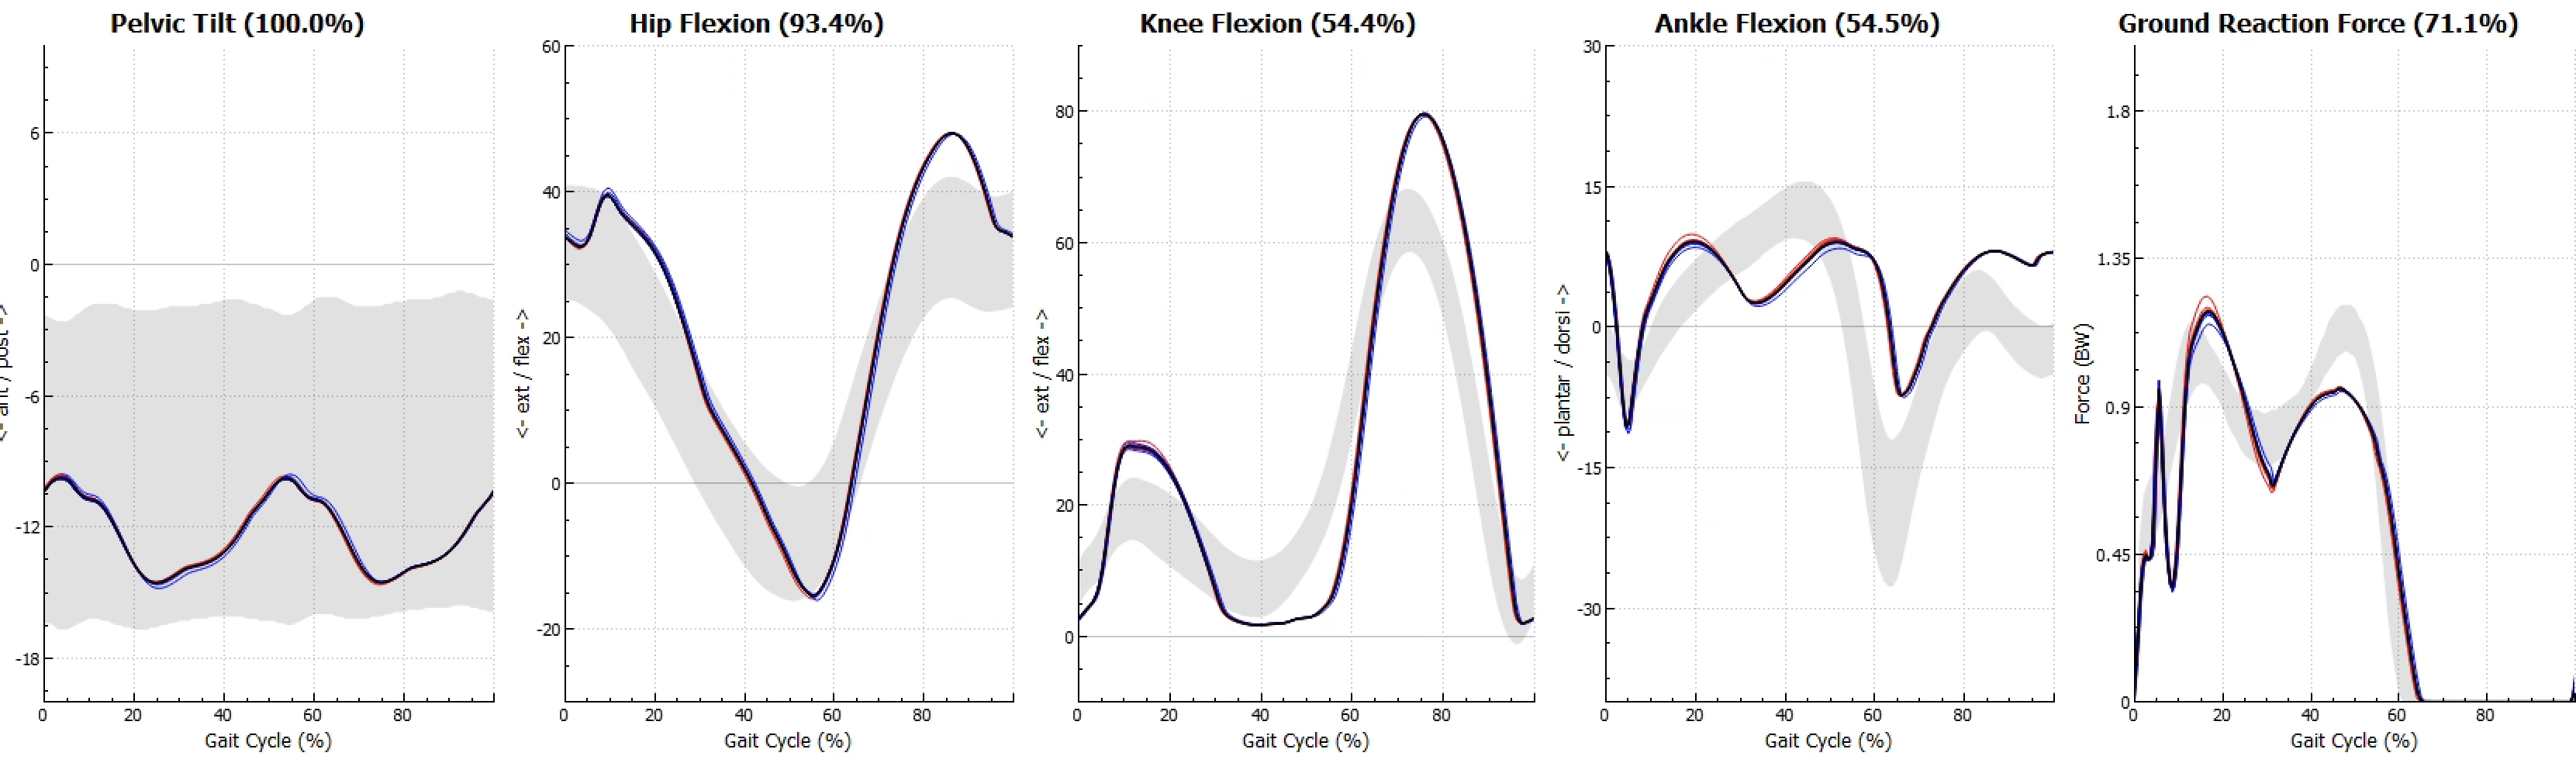
\includegraphics[width=\textwidth]{screens/healthy_gait.png}
    \caption{Gait parameters as observed in the SCONE simulation of the gait of a healthy subject. The grayed-out area show distribution of gait parameters in healthy humans, the colored lines show the gait parameter evolution over multiple gait cycle for our optimal solution.}
    \label{healthy_gait}
\end{figure}

\begin{figure}[h!]
    \centering
    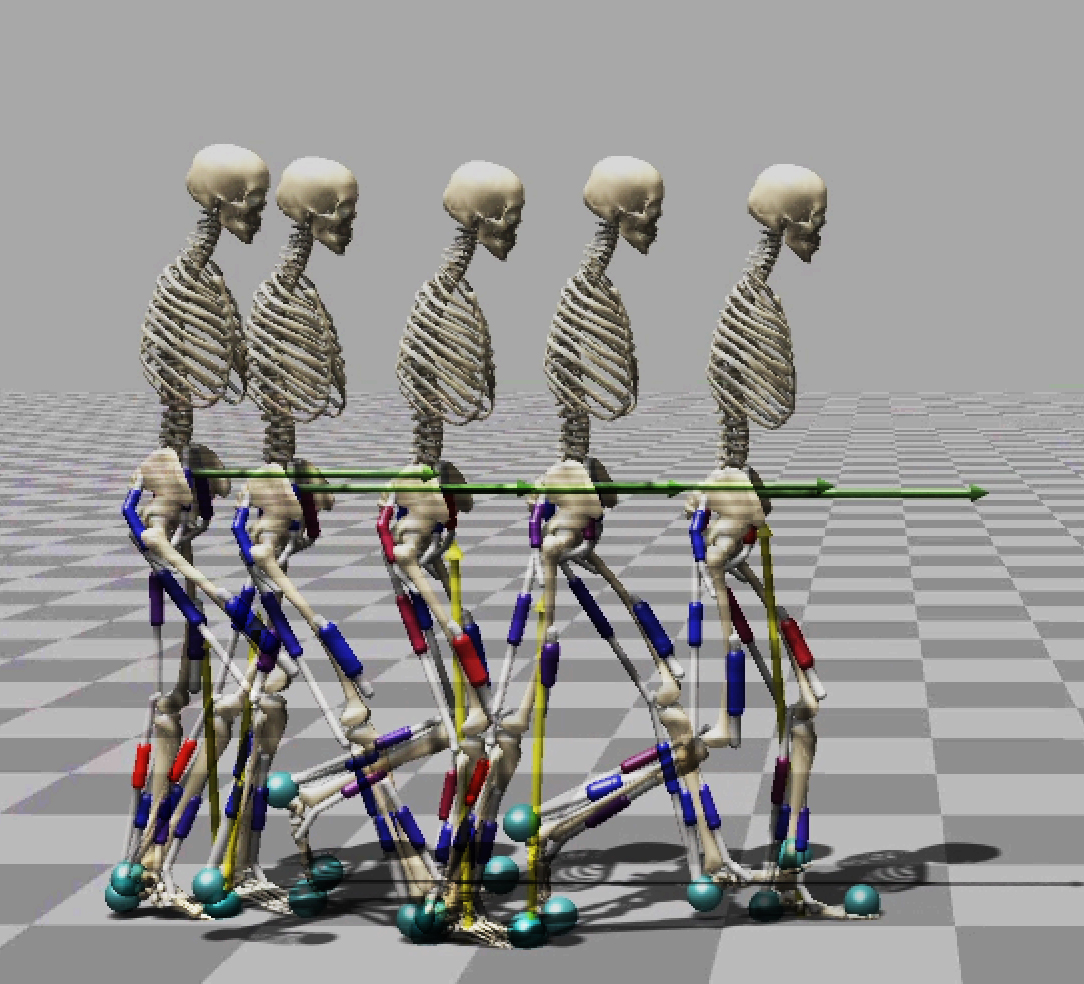
\includegraphics[width=0.4\textwidth]{screens/healthy_walk.jpg}
    \caption{Rendering of the optimization solution produced by the healthy model and controller.}
    \label{healthy_render}
\end{figure}

\section{Pathological Gait : Plantarflexor Muscle Atrophy}

We reduce the maximum force that can be produced by the plantarflexor muscles (\textit{gastrocnemius} and \textit{soleus}). The principal kinetic adaptation is (quite obviously) a reduction of the amplitude of plantarflexion as is clearly visible on 

\begin{figure}[h!]
    \centering
    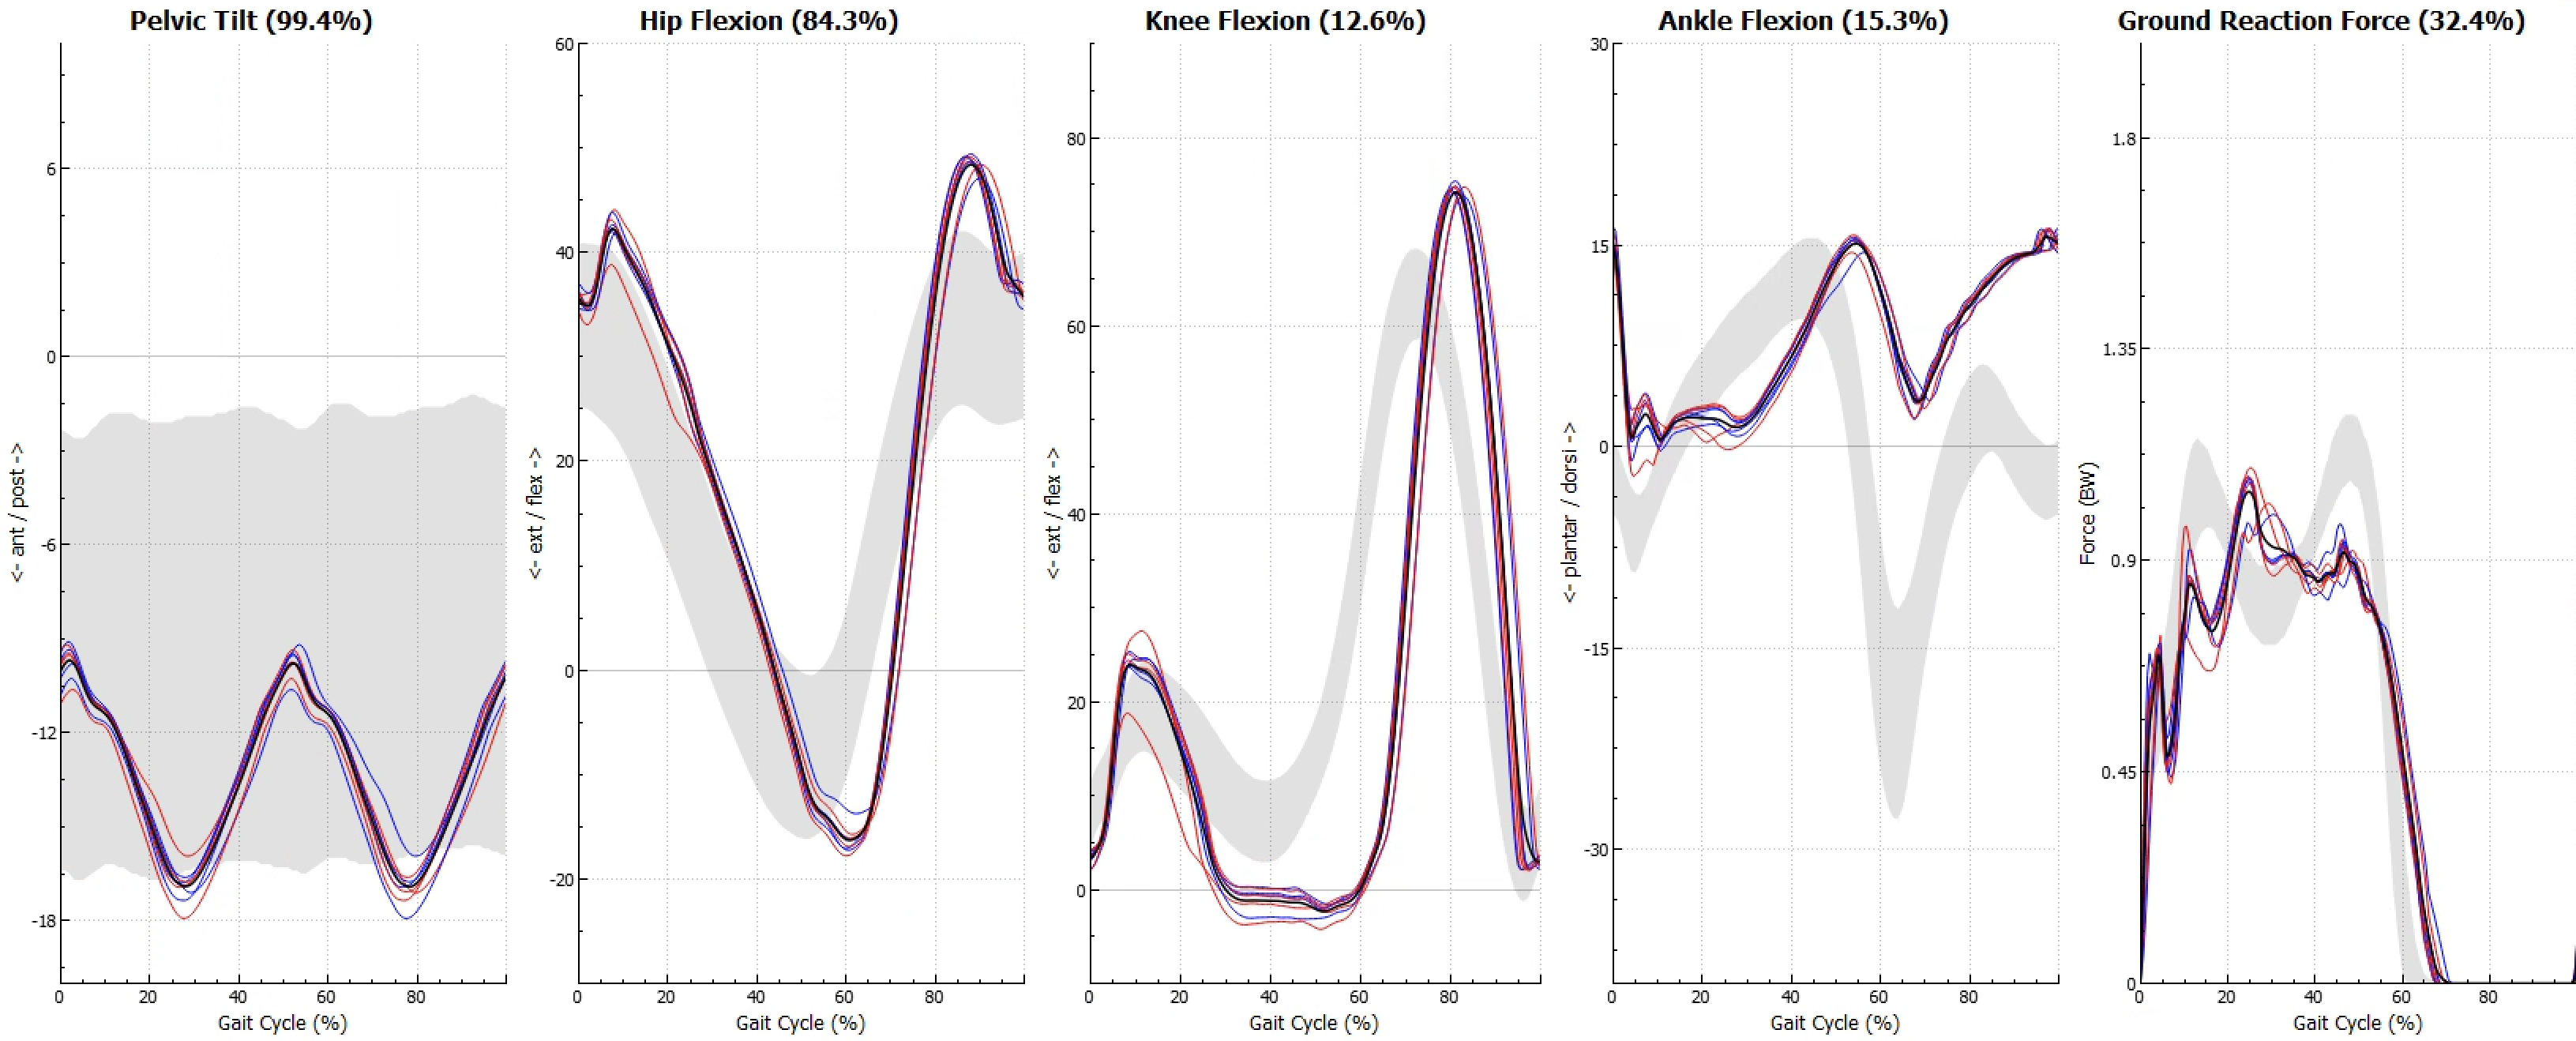
\includegraphics[width=\textwidth]{screens/atrophy_gait.png}
    \caption{Gait parameters as observed in the SCONE simulation of a subject with a gait affected by PF muscular atrophy.}
    \label{atrophic_gait}
\end{figure}

\begin{figure}[h!]
    \centering
    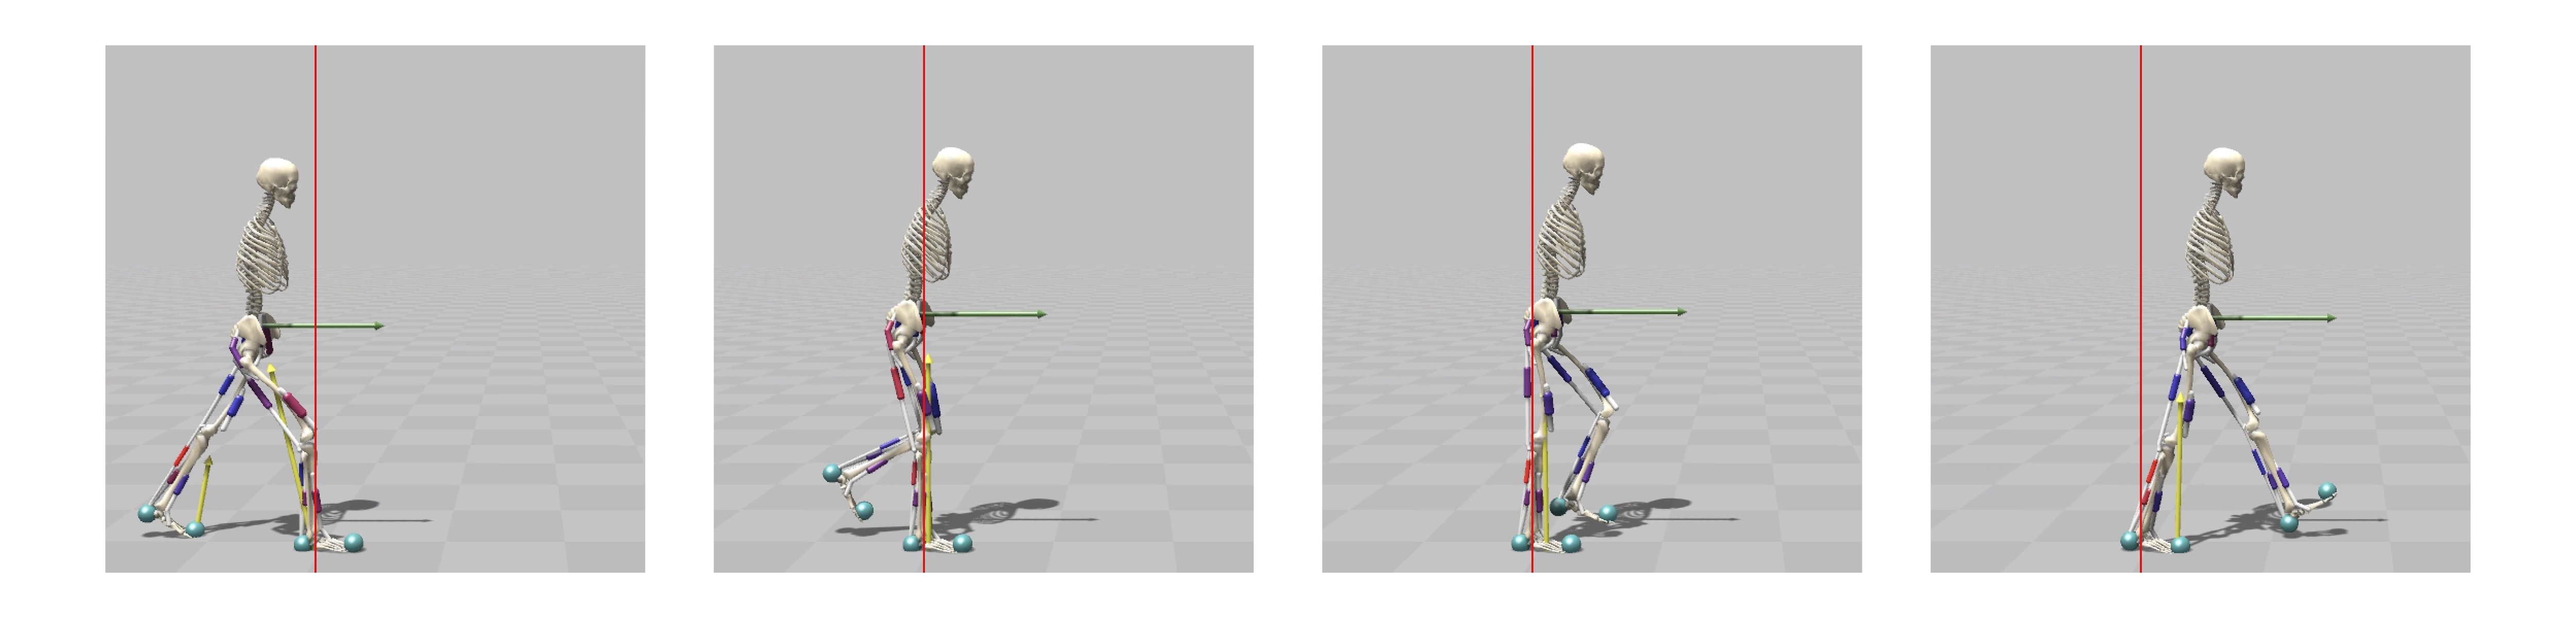
\includegraphics[width=\textwidth]{screens/heel_walk.jpg}
    \caption{Rendering of the optimization solution produced for the PF muscular atrophy model.}
\end{figure}

\section{Pathological Gait : Hyperreflexia}

\begin{figure}[h!]
    \centering
    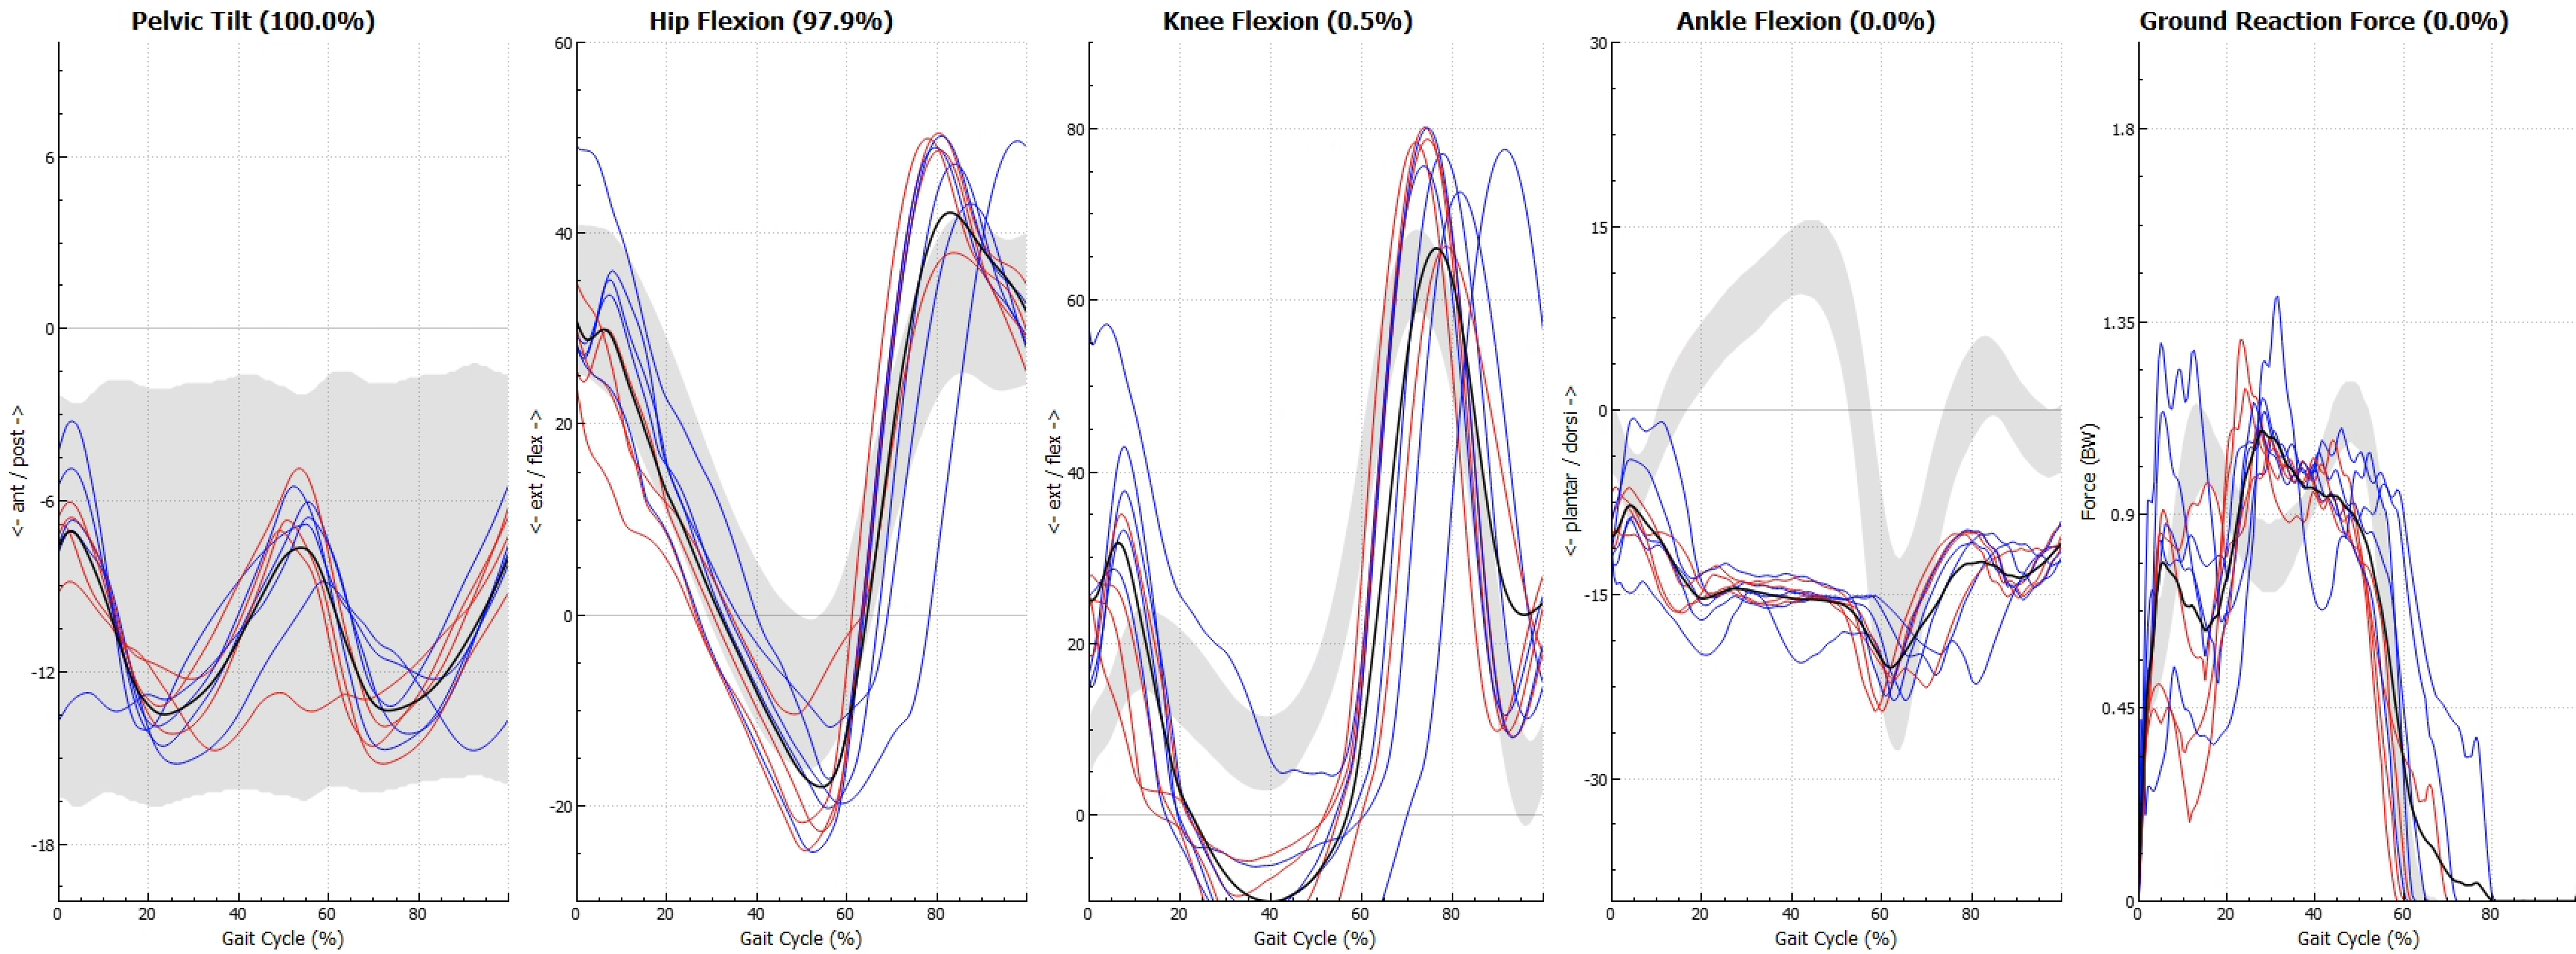
\includegraphics[width=\textwidth]{screens/hyperreflexia_gait.png}
    \caption{Gait parameters as observed in the SCONE simulation of a subject with a gait affected by hyperreflexia.}
\end{figure}

\begin{figure}[h!]
    \centering
    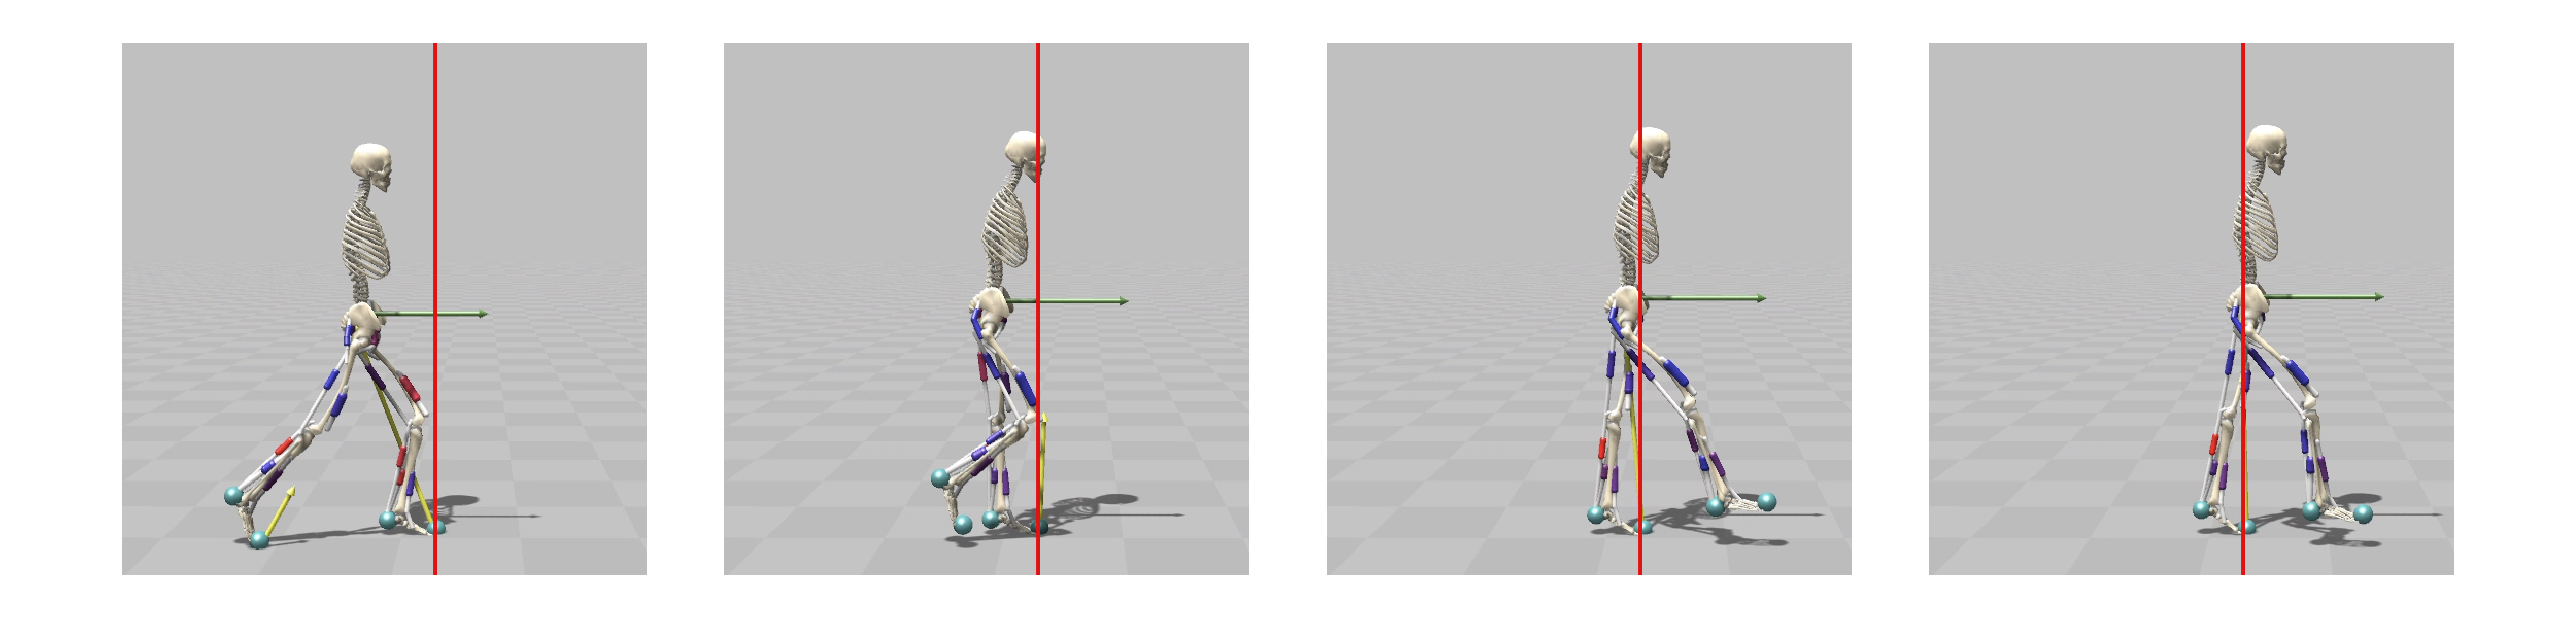
\includegraphics[width=\textwidth]{screens/toe_walk_hr.jpg}
    \caption{Rendering of the optimization solution produced for the hyperreflexia model.}
\end{figure}

\section{Pathological Gait : Heel / Toe Walking}


\end{document}

